\documentclass[10pt,a4paper]{article}

% --- Pakiety ---------------------------------------------------------------
\usepackage{iftex}
\ifXeTeX
  \usepackage{fontspec} % XeTeX/Tectonic: czcionki Unicode (domyślnie Latin Modern)
\else
  \usepackage[utf8]{inputenc}
  \usepackage[T1]{fontenc}
  \usepackage{lmodern}
\fi
\usepackage[polish]{babel}
\usepackage{xcolor}
\usepackage[margin=1.9cm]{geometry}
\usepackage{amsmath,amssymb,mathtools}
\usepackage{graphicx}
\usepackage{booktabs}
\usepackage{listings}
\usepackage{algorithm}
\usepackage{algpseudocode}
\usepackage[font=small,labelfont=bf,skip=3pt]{caption}
\usepackage{enumitem}
\usepackage{microtype}

\setlist{itemsep=1pt,topsep=2pt,parsep=0pt}
\setlength{\parindent}{0pt}
\setlength{\parskip}{3pt}
\renewcommand{\arraystretch}{1.1}

% Styl fragmentów kodu C++
\lstset{
  language=C++,
  basicstyle=\ttfamily\scriptsize,
  keywordstyle=\bfseries,
  commentstyle=\itshape\color[gray]{0.35},
  numbers=left, numberstyle=\tiny, numbersep=4pt,
  frame=single, framerule=0.3pt, rulecolor=\color[gray]{0.6},
  xleftmargin=10pt, aboveskip=3pt, belowskip=3pt,
  columns=fullflexible, keepspaces=true, showstringspaces=false
}

% Pseudokod: polskie słowa kluczowe
\floatname{algorithm}{Algorytm}
\algrenewcommand\algorithmicrequire{\textbf{Wejście:}}
\algrenewcommand\algorithmicensure{\textbf{Wyjście:}}
\algrenewcommand\algorithmicif{\textbf{jeżeli}}
\algrenewcommand\algorithmicthen{\textbf{to}}
\algrenewcommand\algorithmicelse{\textbf{w przeciwnym razie}}
\algrenewcommand\algorithmicreturn{\textbf{zwróć}}
\algrenewtext{EndIf}{\textbf{koniec jeżeli}}
\algrenewtext{If}[1]{\textbf{jeżeli} #1 \textbf{to}}
\algrenewtext{ElsIf}[1]{\textbf{w przeciwnym razie, jeżeli} #1 \textbf{to}}
\algrenewtext{Else}{\textbf{w przeciwnym razie}}
\algrenewtext{Return}{\textbf{zwróć}}

\title{\vspace{-1.2cm}\textbf{Rekurencyjne mnożenie macierzy:\\ metody Binét'a i Strassena}\vspace{-0.3cm}}
\author{Imię Nazwisko (nr albumu) \quad\textbullet\quad Imię Nazwisko (nr albumu)}
\date{\today}

\begin{document}
\maketitle
\vspace{-0.6cm}

\section{Cel i zakres}
Zaimplementowano w C++ dwa rekurencyjne algorytmy mnożenia macierzy kwadratowych
o \emph{dowolnym} rozmiarze $n\times n$ (nie tylko będącym potęgą dwójki): metodę Binét'a (8 mnożeń
bloków) i metodę Strassena (7 mnożeń bloków). Macierze zawierają liczby losowe z rozkładu równomiernego
na przedziale $[10^{-8}, 1)$. Zliczano liczbę operacji zmiennoprzecinkowych $(+,-,*,/)$ oraz mierzono czas
działania. Źródła: \texttt{binet.cpp}, \texttt{strassen.cpp}; skrypty raportowe: \texttt{make\_plots.py},
\texttt{compare.m}.

\section{Pseudokod algorytmów rekurencyjnych}
W obu metodach macierze dzielimy na cztery bloki $A=\begin{psmallmatrix}A_{11}&A_{12}\\A_{21}&A_{22}\end{psmallmatrix}$,
analogicznie $B$ i $C=AB$.

\begin{minipage}[t]{0.495\textwidth}
\begin{algorithm}[H]
\caption{\textsc{Binét}$(A,B)$ (\textsc{B} = wywołanie rekurencyjne)}
\begin{algorithmic}[1]
\Require $A$: $p\times q$, $B$: $q\times r$
\Ensure $C=AB$: $p\times r$
\If{$p=1$ lub $q=1$ lub $r=1$}
  \State \Return \textsc{MnożenieKlasyczne}$(A,B)$
\EndIf
\State $p_h,q_h,r_h \gets \lceil p/2\rceil,\lceil q/2\rceil,\lceil r/2\rceil$
\State podziel $A$ w punktach $(p_h,q_h)$, $B$ w $(q_h,r_h)$
\State $C_{11}\gets \textsc{B}(A_{11},B_{11})+\textsc{B}(A_{12},B_{21})$
\State $C_{12}\gets \textsc{B}(A_{11},B_{12})+\textsc{B}(A_{12},B_{22})$
\State $C_{21}\gets \textsc{B}(A_{21},B_{11})+\textsc{B}(A_{22},B_{21})$
\State $C_{22}\gets \textsc{B}(A_{21},B_{12})+\textsc{B}(A_{22},B_{22})$
\State \Return $\begin{psmallmatrix}C_{11}&C_{12}\\C_{21}&C_{22}\end{psmallmatrix}$
\end{algorithmic}
\end{algorithm}
\end{minipage}\hfill
\begin{minipage}[t]{0.495\textwidth}
\begin{algorithm}[H]
\caption{\textsc{Strassen}$(A,B)$, $n\times n$ (\textsc{S} = wywołanie rekurencyjne)}
\begin{algorithmic}[1]
\If{$n=1$} \State \Return $A\cdot B$ \EndIf
\If{$n$ nieparzyste, $m=n-1$}
  \State wydziel $A_{11}$ ($m{\times}m$), kolumnę $a_{12}$, wiersz $a_{21}$, liczbę $a_{22}$ (tak samo $B$)
  \State $C_{11}\gets \textsc{S}(A_{11},B_{11})+a_{12}b_{21}$
  \State $C_{12}\gets A_{11}b_{12}+a_{12}b_{22}$
  \State $C_{21}\gets a_{21}B_{11}+a_{22}b_{21}$
  \State $C_{22}\gets a_{21}b_{12}+a_{22}b_{22}$
\Else
  \State $M_1\gets \textsc{S}(A_{11}{+}A_{22},\,B_{11}{+}B_{22})$
  \State $M_2\gets \textsc{S}(A_{21}{+}A_{22},\,B_{11})$
  \State $M_3\gets \textsc{S}(A_{11},\,B_{12}{-}B_{22})$
  \State $M_4\gets \textsc{S}(A_{22},\,B_{21}{-}B_{11})$
  \State $M_5\gets \textsc{S}(A_{11}{+}A_{12},\,B_{22})$
  \State $M_6\gets \textsc{S}(A_{21}{-}A_{11},\,B_{11}{+}B_{12})$
  \State $M_7\gets \textsc{S}(A_{12}{-}A_{22},\,B_{21}{+}B_{22})$
  \State $C_{11}\gets M_1{+}M_4{-}M_5{+}M_7$, \; $C_{12}\gets M_3{+}M_5$
  \State $C_{21}\gets M_2{+}M_4$, \; $C_{22}\gets M_1{-}M_2{+}M_3{+}M_6$
\EndIf
\State \Return $C$ złożone z $C_{11},C_{12},C_{21},C_{22}$
\end{algorithmic}
\end{algorithm}
\end{minipage}

\textbf{Dowolny rozmiar.} W metodzie Binét'a przy nieparzystych wymiarach bloki górne/lewe mają
$\lceil\cdot/2\rceil$, a dolne/prawe $\lfloor\cdot/2\rfloor$ wierszy i kolumn, więc mnożymy macierze prostokątne
(wzory na $C_{ij}$ pozostają poprawne). W metodzie Strassena dla nieparzystego $n$ „obieramy'' ostatni wiersz
i kolumnę (\emph{dynamic peeling}); rdzeń $(n{-}1)\times(n{-}1)$ mnożymy rekurencyjnie, a cienkie iloczyny
klasycznie. Macierzy nie dopełniamy zerami, dzięki czemu liczba operacji nie jest sztucznie zawyżona.
Rekurencję prowadzimy do macierzy $1\times1$ (bez progu przełączenia na metodę klasyczną).

\section{Najważniejsze fragmenty kodu}
Licznik operacji zwiększany jest tylko w dwóch miejscach: przy dodawaniu/odejmowaniu macierzy (1 operacja na element)
oraz w mnożeniu klasycznym używanym w przypadku bazowym ($pqr$ mnożeń i $pr(q{-}1)$ dodawań).

\begin{lstlisting}
static unsigned long long g_flops = 0;           // licznik operacji + - * /
Matrix add(const Matrix& A, const Matrix& B) {   // sub() analogicznie
    Matrix C(A.rows, A.cols);
    for (size_t k = 0; k < C.data.size(); ++k) C.data[k] = A.data[k] + B.data[k];
    g_flops += C.data.size();                    // 1 operacja na element
    return C;
}
\end{lstlisting}

\textbf{Binét} (\texttt{binet.cpp}, fragment skrócony):
\begin{lstlisting}
Matrix multiplyBinet(const Matrix& A, const Matrix& B) {
    const int p = A.rows, q = A.cols, r = B.cols;
    if (p == 1 || q == 1 || r == 1) return multiplyNaive(A, B);   // przypadek bazowy
    const int ph = (p + 1) / 2, qh = (q + 1) / 2, rh = (r + 1) / 2;  // punkty podzialu
    Matrix A11 = subMatrix(A, 0, 0, ph, qh), A12 = subMatrix(A, 0, qh, ph, q - qh);
    Matrix A21 = subMatrix(A, ph, 0, p - ph, qh), A22 = subMatrix(A, ph, qh, p - ph, q - qh);
    // ... B11, B12, B21, B22 wycinane analogicznie (wiersze wg qh, kolumny wg rh)
    Matrix C11 = add(multiplyBinet(A11, B11), multiplyBinet(A12, B21));   // 8 mnozen
    Matrix C12 = add(multiplyBinet(A11, B12), multiplyBinet(A12, B22));
    Matrix C21 = add(multiplyBinet(A21, B11), multiplyBinet(A22, B21));
    Matrix C22 = add(multiplyBinet(A21, B12), multiplyBinet(A22, B22));
    // ... sklejenie C11..C22 w macierz wynikowa p x r (placeBlock)
}
\end{lstlisting}

\textbf{Strassen} (\texttt{strassen.cpp}, fragment skrócony):
\begin{lstlisting}
Matrix multiplyStrassen(const Matrix& A, const Matrix& B) {
    const int n = A.rows;
    if (n <= STRASSEN_CUTOFF) return multiplyNaive(A, B);   // CUTOFF = 1
    if (n % 2 == 1) {                                        // obieranie: m = n-1 parzyste
        // ... A11 (m x m), a12, a21, a22 oraz b.. wycinane przez subMatrix
        Matrix C11 = add(multiplyStrassen(A11, B11), multiplyNaive(a12, b21));
        // ... C12, C21, C22: tylko "cienkie" iloczyny multiplyNaive + add
    }
    // n parzyste: 7 mnozen rekurencyjnych zamiast 8
    Matrix M1 = multiplyStrassen(add(A11, A22), add(B11, B22));
    Matrix M2 = multiplyStrassen(add(A21, A22), B11);
    Matrix M3 = multiplyStrassen(A11, sub(B12, B22));
    Matrix M4 = multiplyStrassen(A22, sub(B21, B11));
    Matrix M5 = multiplyStrassen(add(A11, A12), B22);
    Matrix M6 = multiplyStrassen(sub(A21, A11), add(B11, B12));
    Matrix M7 = multiplyStrassen(sub(A12, A22), add(B21, B22));
    Matrix C11 = add(sub(add(M1, M4), M5), M7);   Matrix C12 = add(M3, M5);
    Matrix C21 = add(M2, M4);                     Matrix C22 = add(add(sub(M1, M2), M3), M6);
    // ... sklejenie C11..C22 w macierz wynikowa n x n
}
\end{lstlisting}

\section{Środowisko pomiarowe}
\textbf{Język nie jest interpretowany:} C++ jest kompilowany z góry do natywnego kodu maszynowego x86-64
(\texttt{g++ 14.2.0}, MinGW-W64, flagi \texttt{-O2 -std=c++17}); powstały plik \texttt{.exe} jest wykonywany
bezpośrednio przez procesor, bez interpretera i maszyny wirtualnej. Obliczenia były jednowątkowe.
\textbf{Sprzęt:} procesor AMD Ryzen 7 7735HS (8 rdzeni / 16 wątków, taktowanie bazowe 3,2~GHz),
pamięć RAM 31,2~GB DDR5 (4800~MT/s), system Windows 11. Czas mierzono zegarem \texttt{std::chrono::steady\_clock}
tylko dla samego mnożenia (bez generowania macierzy i weryfikacji): dla $n\le200$ jako minimum z 3~powtórzeń,
dla $n>200$ jako pojedynczy pomiar (programy uruchamiane kolejno; dla $n\le200$ oba programy liczyły równocześnie na osobnych rdzeniach). Pomiary czasu wykonano dla $n=1,2,\dots,200$ oraz $n=250,300,\dots,1000$ (krok 50);
liczbę operacji wyznaczono dla \emph{każdego} $n=1,\dots,1000$, korzystając z modelu rekurencyjnego (to samo drzewo
wywołań co w algorytmie, ale bez mnożenia macierzy). Dla wszystkich zmierzonych $n$ model daje liczbę operacji
identyczną z licznikiem w działającym programie. Maksymalny rozmiar, który udało się policzyć obiema metodami: $n=1000$.

\section{Wykresy}
\begin{figure}[H]
\centering
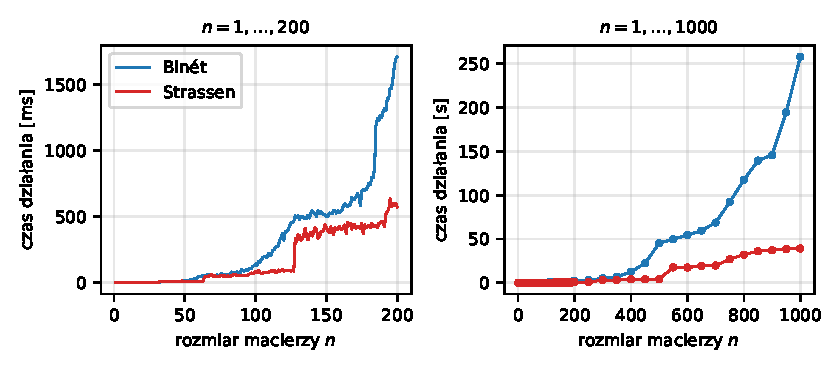
\includegraphics[width=0.86\textwidth]{fig_time.pdf}
\caption{Czas działania obu metod rekurencyjnych w zależności od rozmiaru macierzy $n$.}
\label{fig:time}
\end{figure}

\begin{figure}[H]
\centering
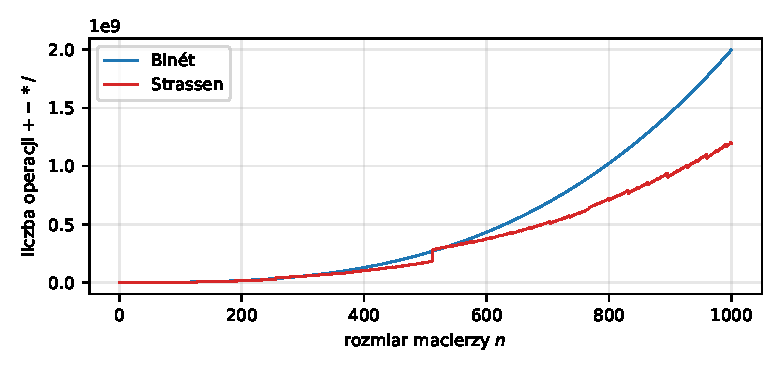
\includegraphics[width=0.78\textwidth]{fig_flops.pdf}
\caption{Liczba operacji zmiennoprzecinkowych $(+,-,*,/)$ w zależności od $n$, $n=1,\dots,1000$.}
\label{fig:flops}
\end{figure}

\textbf{Komentarz.} Liczba operacji w metodzie Binét'a wynosi dokładnie $2n^3-n^2$ (dla $n=1000$:
$1\,999\,000\,000$), czyli tyle samo co w algorytmie klasycznym. Strassen dla małych $n$ wykonuje \emph{więcej}
operacji (1,92$\times$ dla $n=16$, 1,01$\times$ dla $n=100$), bo rekurencja aż do macierzy $1\times1$ generuje
wiele dodawań macierzy; dla $n\ge 536$ ma już zawsze mniej operacji niż Binét (dla $n=1000$: $1\,199\,169\,602$,
czyli 60\% operacji Binét'a). Wykres Strassena jest „schodkowy'': tuż po przekroczeniu potęgi dwójki
(np. $n=511\to512$: z $1{,}83\cdot10^{8}$ do $2{,}81\cdot10^{8}$ operacji) rekurencja schodzi o jeden poziom głębiej.
Czas działania zależy nie tylko od liczby operacji, ale też od kopiowania i alokacji macierzy tymczasowych oraz
od pamięci podręcznej -- stąd skoki na rys.~\ref{fig:time}. Dla $n=1000$ Strassen potrzebuje ok.\ 39~s, a Binét
ok.\ 258~s (6,6 razy dłużej), mimo że liczby operacji różnią się tylko 1,7 raza: Binét tworzy więcej macierzy
tymczasowych (8 wywołań rekurencyjnych na poziom zamiast 7).

\section{Oszacowanie złożoności obliczeniowej}
\textbf{Teoretycznie.} Binét: $T(n)=8T(n/2)+\Theta(n^2)$, więc z twierdzenia o rekurencji uniwersalnej
$T(n)=\Theta(n^{\log_2 8})=\Theta(n^3)$; dokładnie $2n^3-n^2$ operacji (zgodnie z danymi dla każdego
$n=1,\dots,1000$). Strassen: $S(n)=7S(n/2)+18(n/2)^2$, więc $S(n)=\Theta(n^{\log_2 7})\approx\Theta(n^{2{,}807})$;
dla $n=2^k$ dokładnie $S(n)=7\,n^{\log_2 7}-6\,n^2$ (sprawdzone dla $k=0,\dots,9$; np. $n=4$: 247 operacji).

\textbf{Eksperymentalnie} (rys.~\ref{fig:loglog}): dopasowanie prostej do danych w skali log-log daje wykładnik
$\alpha$ w zależności $\sim n^{\alpha}$.
Dla liczby operacji: Binét $\alpha=3{,}00$, Strassen $\alpha=2{,}80$ ($n\ge16$, wszystkie $n$; dla samych $n=2^k$
wychodzi $2{,}87$, nieco więcej niż $2{,}807$, bo dla małych $n$ ważny jest składnik $-6n^2$).
Dla czasu ($n\ge50$): Binét $\alpha=3{,}16$, Strassen $\alpha=2{,}85$. Czas rośnie nieco szybciej niż liczba operacji
ze względu na efekty pamięci. \textbf{Wniosek:} Binét ma złożoność $O(n^3)$, Strassen $O(n^{\log_2 7})\approx O(n^{2{,}81})$;
przewaga Strassena rośnie z $n$, ale przy rekurencji do $1\times1$ ujawnia się dopiero dla $n$ rzędu kilkuset.

\begin{figure}[H]
\centering
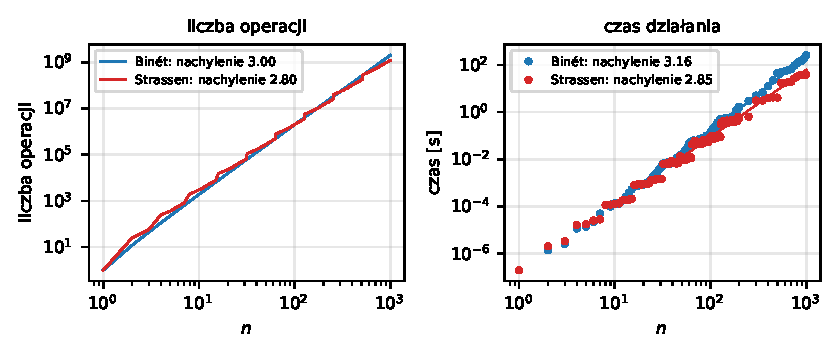
\includegraphics[width=0.86\textwidth]{fig_loglog.pdf}
\caption{Wykresy w skali log-log; nachylenie dopasowanej prostej oznacza wykładnik $\alpha$ w zależności $\sim n^{\alpha}$.}
\label{fig:loglog}
\end{figure}

\section{Przykład $4\times4$ -- porównanie z Octave/MATLAB}
Do porównania wybrano $A=\texttt{magic(4)}$, $B=A^{T}/7$ (te same macierze są zaszyte w trybie
\texttt{--example} obu programów). Skrypt \texttt{compare.m} wczytuje wyniki programów C++ i porównuje je z $A*B$
w Octave/MATLAB. Wynik referencyjny:
\[
C_{\mathrm{ref}} = A B \approx
\begin{pmatrix}
62{,}5714 & 33{,}7143 & 47{,}4286 & 21{,}4286\\
33{,}7143 & 44{,}2857 & 39{,}7143 & 47{,}4286\\
47{,}4286 & 39{,}7143 & 44{,}2857 & 33{,}7143\\
21{,}4286 & 47{,}4286 & 33{,}7143 & 62{,}5714
\end{pmatrix}.
\]
\begin{center}
\begin{tabular}{lcc}
\toprule
metoda & liczba operacji & $\max|C-C_{\mathrm{ref}}|$ \\
\midrule
Binét & 112 $(=2\cdot4^3-4^2)$ & $7{,}1\cdot10^{-15}$ \\
Strassen & 247 $(=7\cdot7^2-6\cdot4^2)$ & $1{,}4\cdot10^{-14}$ \\
\bottomrule
\end{tabular}
\end{center}
Obie metody dają wynik zgodny z mnożeniem wbudowanym z dokładnością do błędów zaokrągleń (rzędu $10^{-14}$);
Strassen ma nieco większy błąd, bo wykonuje więcej dodawań/odejmowań w innej kolejności.
% UWAGA: wartości referencyjne w tej wersji wyznaczono równoważnym wywołaniem A @ B w NumPy.
% Po uruchomieniu compare.m w Octave/MATLAB sprawdź, czy błędy w tabeli się zgadzają.

\end{document}
